\documentclass[a4paper,english, 10pt, twoside]{article}
\usepackage[utf8]{inputenc}
\usepackage[T1]{fontenc}
\usepackage[english]{babel}
\usepackage{epsfig}
\usepackage{graphicx}
\usepackage{amsfonts, amssymb, amsmath}
\usepackage{listings}
\usepackage{float}
\usepackage[top=2cm, bottom=2cm, left=2cm, right=2cm]{geometry}
\renewcommand{\d}{\partial}
%opening
\title{Project 5, FYS4150}
\author{Candidate 55}


\begin{document}

\maketitle
\newpage
\tableofcontents
\newpage
\section{About the problem}
In this project we will look at the transportation of neurotransmitter molecules across the so called synaptic cleft separating a 
brain cell and a target cell. After an ``action-potential'' is recieved (in the axon terminal) vesicles inside the axon terminal merge with the 
presynaptic membrane, releasing the neurotransmitter molecules into the synaptic cleft. 
A vesicle is a kind of ``bubble'' inside a cell. Here we are talking about vesicles containing neurotransmitter moleules located in the axon (or 
nerve fibers) of a brain cell. The molecules then diffuse across the synaptic cleft, and are picked up by receptors on the target cell (or the 
postsynaptic side of the synaptic cleft if you want). We want to modell this particular event using a continuum modell, and the mathematical 
expression is the diffusion equation.
\begin{equation*}
{\d u \over \d t} = D\nabla^2 u 
\end{equation*}
Where D is a diffusion coefficient. An illustrative figure of the problem can be found in figure (\ref{synapse}).
\begin{figure}[H]
 \centering
 \includegraphics[scale = 0.7]{Chemical_synapse_schema.jpg}
 \caption{Illustration of communication between two brain cells and a close-up of the synaptic cleft separating the axon (presynaptic side) and
 the target cell (postsynaptic side). (From wikipedia search Chemical synapse) }
 %http://en.wikipedia.org/wiki/Chemical_synapse
 \label{synapse}
\end{figure}
We will assume that the synaptic cleft is of roughly equal width, and that the area of the synaptic cleft is large compared to its width. The 
concentration of neurotransmitters therefore only vary in one direction, from presynaptic to postsynaptic side. The diffusion equation then reduces 
to
\begin{equation*}
 {\d u \over \d t} = D{\d^2 u \over \d x^2}
\end{equation*}
which we can rescale to be dimensionless by introducing $x = \alpha\tilde{x} $
\begin{equation*}
 {\d u \over \d t} = D{\d^2 u \over \alpha^2\d\tilde{x}^2}
\end{equation*}
and define $\alpha^2 = D; \; \tilde{x} = x$ giving us the diffusion equation in its simplest form.
\begin{equation*}
 {\d u \over \d t} = {\d^2 u \over \d x^2}
\end{equation*}
We will say that at some time $t = 0$ the ``action potential'' is recieved, and the vesicles merge with the presynaptic membrane meaning that the 
initial distribution of neurotransmitters is $u(x,0) = \delta(x)$, that is 1 at $x = 0$ and 0 everywhere else. Furthermore we say that the 
neurotransmitters which reach the postsynaptic membrane (or the receptors) are removed from the synaptic cleft (and our system). This means that at 
the far side ($x=d$) $u(d,t) = 0$. We are now ready to solve the equation, see sections \ref{numerical} and \ref{analytic}.\\
We will also extend the diffusion equation to two spatial dimensions, also using dimensionless variables. The boundary and initial conditions of 
the two dimensional equation are quite different from the one dimensional case. We use $x,y\in[0,1]$,
$$
u(x,y,0) = (1-y)e^{x}
$$
and
\begin{align*}
 u(0,y,t) &= (1-y)e^{t} \\
 u(1,y,t) &= (1-y)e^{1+t} \\
 u(x,0,t) &= e^{x+t} \\
 u(x,1,t) &= 0
\end{align*}

\subsection{Notation}
For finite differences I will use the the notation 
\begin{equation*}
 u(t_n,x_i,y_j) = u^n_{i,j}
\end{equation*}
where $t_n = t_0 + n\cdot\Delta t$, $x_i = x_0 +i\cdot\Delta x$ and $y_j = y_0 +j\cdot\Delta y$. Thus it is important not to 
confuse $u^n$ (u to the power of n) with $u^n_{i,j}$ (u evaluated at timestep n and position i,j). I will at some points use the 
matrix B to simplify writing. B is defined to be
\begin{align*}
 \mathbf{B} = \left(\begin{array}{c c c c c c c}
        2 & -1 &0 &\dots & &0 &0 \\
        -1 & 2 & -1 &0 &\dots & &0 \\
        0& \ddots & \ddots & \ddots &  &  &0\\
        0& \dots &  &0&-1 & 2 & -1\\
         0& \dots & & &0&-1 & 2 
       \end{array}\right)
\end{align*}
\section{The algorithm}\label{numerical}
We will solve the 1+1 dimensional difusion equation by three different finite differnce schemes in this project. Using the 
standard approximation of the second derivative in space, we use successively more elaborate approximations to the time derivative. 
\subsection{Forward Euler}
Starting off with the Forward Euler (FE) approximation we get the following scheme
\begin{align*}
 \frac{u^{n+1}_i-u^n_i}{\Delta t} = \frac{u^n_{i+1}-2u^n_i + u^n_{i-1}}{\Delta x^2}
\end{align*}
\begin{equation}\label{FE}
 u^{n+1}_i = \frac{\Delta t}{\Delta x^2}\left(u^n_{i+1}-2u^n_i + u^n_{i-1}\right) +u^n_i
\end{equation}
So to solve the equation all we have to do is loop over the two variables and we are done.\\
\begin{lstlisting}
for n = 0,1, ... , N
    for i = 0,1, ... , N_x
	u_new[i] = dtdx2*(u_prev[i+1]-2*u_prev[i] + u_prev[i-1]) + u_prev[i];
    u_prev = u_new;
end;
\end{lstlisting}

A discussion of stability and the error in this scheme can be found in the ``Stability and precision'' section.
\subsection{Backward Euler}
The Backward Euler (BE) approximation gives us a slightly more elaborate scheme seeing at it is an implicit one. The discretization 
gives
\begin{align*}
 \frac{u^{n}_i-u^{n-1}_i}{\Delta t} = \frac{u^n_{i+1}-2u^n_i + u^n_{i-1}}{\Delta x^2} \\
 u^n_i -\frac{\Delta t}{\Delta x^2}\left(u^n_{i+1}-2u^n_i + u^n_{i-1}\right) = u^{n-1}_i \\
 u^n_i\Big(1+2\dfrac{\Delta t}{\Delta x^2}\Big) -u^n_{i-1}\dfrac{\Delta t}{\Delta x^2} - u^n_{n+1}\dfrac{\Delta t}{\Delta x^2} 
 = u^{n-1}_i
\end{align*}
If we insert for a few steps we see that this takes the form of
\begin{align}\label{BE}
 \left(\begin{array}{c c c c c c c c}
        \Big(1+2\dfrac{\Delta t}{\Delta x^2}\Big) & -\dfrac{\Delta t}{\Delta x^2} &0 &\dots & & &0 &0 \\
        -\dfrac{\Delta t}{\Delta x^2} & \Big(1+2\dfrac{\Delta t}{\Delta x^2}\Big) & -\dfrac{\Delta t}{\Delta x^2} &0 &\dots & & &0 \\
        0& \ddots & \ddots & \ddots & 0 & \dots &  &0\\
        0& \dots & & &0&-\dfrac{\Delta t}{\Delta x^2} & \Big(1+2\dfrac{\Delta t}{\Delta x^2}\Big) & -\dfrac{\Delta t}{\Delta x^2}\\
         0& \dots & && &0&-\dfrac{\Delta t}{\Delta x^2} & \Big(1+2\dfrac{\Delta t}{\Delta x^2}\Big) 
       \end{array}\right)\mathbf{u}^n = \mathbf{u}^{n-1} 
\end{align}
\begin{equation*}
 \mathbf{A}\mathbf{u}^n = \mathbf{u^{n-1}}
\end{equation*}

So for each timestep we need to multiply the inverse of $\mathbf{A}$ with a vector $\mathbf{u}^{n-1}$ containig the solution at 
the previous timestep. Looking a bit closer at equation (\ref{BE}) we realize two things. First of all, the matrix 
$\mathbf{A}$ does'nt change at all throughout the computation so we can get away with invertig it once. Second, and perhaps 
more important, we allready have a very efficient solver for this kind of problem from project 1.\\

A discussion of stability and the error in this scheme can be found in the ``Stability and precision'' section.

\subsection{Crank Nicolson}
Finally, we can use the Crank Nicolson approximation of the time derivative which is a special case of the so called theta -rule 
with $\theta = 0.5$.
\begin{align*}
 \frac{u^n_i - u^{n-1}_i}{\Delta t} = \frac{1}{2\Delta x^2}\Big(u^n_{i+1} -2u^n_{i} + u^n_{i-1}\Big) +\frac{1}{2\Delta x^2}
 \Big(u^{n-1}_{i+1} -2u^{n-1}_{i} + u^{n-1}_{i-1}\Big) \\
 u^n_i -\frac{\Delta t}{2\Delta x^2}\Big(u^n_{i+1} -2u^n_{i} + u^n_{i-1}\Big) = u^{n-1}_i + 
 \frac{\Delta t}{2\Delta x^2}\Big(u^{n-1}_{i+1} -2u^{n-1}_{i} + u^{n-1}_{i-1}\Big)\\
 u^n_i(2+2C) - Cu^n_{i+1} - Cu^n_{i-1} = u^{n-1}_i(2-2C) + Cu^{n-1}_{i+1} + Cu^{n-1}_{i-1}
\end{align*}
where $C = \frac{\Delta t}{\Delta x^2}$. This can also be expressed as a linear algebra problem
\begin{equation}\label{CN}
 (2\mathbf{I}+C\mathbf{B})\mathbf{u}^n = (2\mathbf{I}-C\mathbf{B})\mathbf{u}^{n-1}
\end{equation}
Again we observe that we will need to invert a matrix, but this time we will also need to do a matrix-vector multiplication.
\begin{align*}
 (2\mathbf{I}+C\mathbf{B})\mathbf{u}^n = (2\mathbf{I}-C\mathbf{B})\mathbf{u}^{n-1} = \tilde{\mathbf{u}}^{n-1}\\
 \mathbf{u}^n = (2\mathbf{I}+C\mathbf{B})^{-1}\tilde{\mathbf{u}}^{n-1}
\end{align*}
This is the same problem as we had in the BE case, only with a modified right-hand side

\subsection{2+1 dimensional diffusion equation}

The Jacobi algorithm for solving linear systems is an iterative scheme very well suited for solving the Poisson and Laplace 
equations in 2 or 3 dimensions. If we breefly look at the discretization of the Laplace equation in 2D (\ref{laplace}) we see that 
there is no obvious way to solve for a new point since we do not know 3 out of 5 points needed to calculate a new one. The solution 
is then (since there is no initial condition either) to start out with an educated guess, and use the scheeme (\ref{laplace scheme}) 
point by point on the entire grid several times until the solution (hopefully) converges.
\begin{align*}
 \nabla^2u(x,y) = 0\\
 \frac{\partial^2 u}{\partial x^2} +  \frac{\partial^2 u}{\partial y^2} = 0 
\end{align*}
\begin{equation}\label{laplace}
 \frac{u_{i+1,j}-2u_{i,j}+u_{i-1,j}}{\Delta x^2} +  \frac{u_{i,j+1}-2u_{i,j}+u_{i,j-1}}{\Delta y^2} = 0
\end{equation}
\begin{equation}\label{laplace scheme}
u_{i,j} = \frac{1}{4}\Big(u_{i-1,j}+u_{i+1,j}+u_{i,j-1}+u_{i,j+1}\Big) 
\end{equation}
Where we have assumed that $\Delta x = \Delta y$. Seeing as we have a time dependence, we also have an initial condition on our 
system. Therefore we allready know all values at previous timesteps (since the sceme is recursive), and we do not have to start 
with a quess of what the solution might look like. In stead, but still with the mentality of the Jacobi algorithm of using the 
previous value to get the new one, we can simply derive an explicit scheme by inserting our approximate derivatives. For example 
if we approximate the time derivative using the FE method we get
\begin{align*}
 \frac{u^{n+1}_{i,j}-u^n_{i,j}}{\Delta t} = \frac{u^n_{i+1,j}-2u^n_{i,j} + u^n_{i-1,j}}{\Delta x^2}+ 
 \frac{u^n_{i,j+1}-2u^n_{i,j} + u^n_{i,j-1}}{\Delta y^2} \\
 u^{n+1}_{i,j} = \frac{\Delta t}{\Delta x^2}\big(u^n_{i+1,j}-2u^n_{i,j} + u^n_{i-1,j}\big) + 
 \frac{\Delta t}{\Delta y^2}\big(u^n_{i,j+1}-2u^n_{i,j} + u^n_{ij-1}\big) + u^n_{i,j}
\end{align*}
This is the same scheme as in \ref{FE} only with one more dimension. As we will se in the ``stability and precision'' section 
the centered difference or ``Leap Frog'' scheme has a better truncation error with respect to time than the FE scheme, and this 
will therefore (most likely) yield better results. The Leap Frog scheme is

\begin{align*}
 \frac{u^{n+1}_{i,j}-u^{n-1}_{i,j}}{2\Delta t} = \frac{u^n_{i+1,j}-2u^n_{i,j} + u^n_{i-1,j}}{\Delta x^2}+ 
 \frac{u^n_{i,j+1}-2u^n_{i,j} + u^n_{i,j-1}}{\Delta y^2}\\
  u^{n+1}_{i,j} = \frac{\Delta t}{2\Delta x^2}\big(u^n_{i+1,j}-2u^n_{i,j} + u^n_{i-1,j}\big) + 
 \frac{\Delta t}{2\Delta y^2}\big(u^n_{i,j+1}-2u^n_{i,j} + u^n_{ij-1}\big) + u^{n-1}_{i,j}
\end{align*}

We could also make an explicit scheme by the mentality in the Gauss-Seidel algorithm. That is to use some of the new values to get 
a new value. In one dimension this is known as the Euler-Chromer method and is known to be quite good for its simplicity. If we 
look closer at the FE or Leap Frog scheme we notice that we allready know the values $u^{n+1}_{i-1,j}$ and $u^{n+1}_{i,j-1}$. 
Using these values might give us better accuracy (at least compared to the FE case)
\section{Analytic solution}\label{analytic}
As a comparison we can find the analytic solution to this problem as follows. 
 \begin{align}\label{eq}
  &\frac{\partial u}{\partial t} = D\frac{\partial^2 u}{\partial x^2}, \,\,\,\,\, u(x,0) = u(d,t) = 0\\
  &x\in[0,d],\,\,\,\,\,\, D = d = u(0,t) = 1
 \end{align}
We see right away that the boundary $x=0$ could give us some problems, so we start off with a small trick
$$
u(x,t) = v(x,t) = u(x,t) - u_s(x)
$$
where the $u_s = 1-x$ term is the steady-state solution to equation \ref{eq}. This trick leaves us with new boundary conditions 
un $u(x,t)$ 
$$
v(0,t) = u(0,t) - u_s(0,t) = 1, \;\; u_s(0,t) = 1 \implies u(0,t) = 0
$$
which makes the whole procedure much simpler. We now assume that $u(x,t)$ can be separated into factors 
\begin{align*}
&u(x,t) = F(x)G(t) \implies \frac{\partial u}{\partial t} = \frac{\partial^2 u}{\partial x^2} \to F(x)\frac{\partial G}{\partial t}
= G(t)\frac{\partial^2 F}{\partial x^2}\\
&\frac{1}{G(t)}\frac{\partial G}{\partial t} =-k^2 =  \frac{1}{F(x)}\frac{\partial^2 F}{\partial x^2}
\end{align*}
We start with the simplest of the equations which is the time dependence
\begin{align*}
 \frac{1}{G(t)}\frac{\partial G}{\partial t} =-k^2\\
 G(t) =C e^{-k^2t}
\end{align*}
and leave it like this for now. The x-dependent equation is somewhat more complicated
\begin{align*}
 \frac{1}{F(x)}\frac{\partial^2 F}{\partial x^2} = -k^2 \\
 F(x) = A\sin(kx) + B\cos(kx)
\end{align*}
\begin{align*}
 F(0) = A\sin(0) + B\cos(0) = 0 \implies B= 0\\
 F(d) = A\sin(kd) = 0 \implies k = \frac{m\pi}{d} = \pi m, \;\; A = A_m
\end{align*}
we now combine all the equations to determine $v(x,t)$
\begin{align*}
 v(x,t) = 1-x + \sum\limits_{m=1}^{\infty}B_me^{-(m\pi)^2t}\sin(m\pi x) \\
 v(x,0) = 1-x +\sum\limits_{m=1}^{\infty}B_m\sin(m\pi x)\\
 \implies \int\limits_0^1\sin(m\pi x)\sin(n\pi x)dx = \delta_{mn} = \int\limits_0^1(x-1)\sin(m\pi x)dx = -\frac{2}{m\pi} = B_m
\end{align*}
This gives us the full analytical solution 
\begin{equation}\label{solution}
 v(x,t) = 1-x-\frac{2}{\pi}\sum\limits_{m = 1}^{\infty}\frac{1}{m}e^{-(m\pi)^2t}\sin(m\pi x) 
\end{equation}
which satisfies all initial and boundary conditions.
\section{Results/Verification}
From section \ref{analytic} we have the analytic solution to our problem, and we can use this to verify our numerical schemes. Now we know from 
section \ref{stability} that both the FE and the BE schemes have errors going like $\mathcal{O}(\Delta t)$, and that the FE scheme has a stability 
criterion of $\Delta t\leq {\Delta x^2 \over 2}$. From experience I know that using exactily this criterion can be bad, so we will use half of this 
and we will use the same for all the schemes so that we can easily compare results. In the analytic solution we have an infinite sum, which we of 
course have to cut at some point. Looking at our solution (\ref{solution}) we see that $t=0$ will have the slowest convergence because there will be 
no additional dampening term in the exponential term. From figure (\ref{convergence_analytic}) we see that there is very little change in afer 25 
terms. It will then be very safe to terminate the sum after some 100-200 terms to make sure no ``invisible'' roundoffs are made.
\begin{figure}[H]
 \centering
 \includegraphics[scale = 0.7]{series_convergence_t0.png}
 \caption{Plot of the analytic solution at $t=0$ while adding more terms. }
 \label{convergence_analytic}
\end{figure}
The errors we get from the different schemes have been visualized in figures (\ref{errors_nx10}) and (\ref{errors_nx100}). As mentioned the error 
should go like $\mathcal{O}(\Delta t)$. 
%Both the anticipated and the real errors can be found in table ()
\begin{figure}[H]
 \centering
 \includegraphics[scale = 0.7]{error_plot_x10.png}
 \caption{The absolute error for $\Delta x = ^1/_{10}$. }
 \label{errors_nx10}
\end{figure}
\begin{figure}[H]
 \centering
 \includegraphics[scale = 0.7]{error_plot_x100.png}
 \caption{The absolute error for $\Delta x = ^1/_{100}$. }
 \label{errors_nx100}
\end{figure}
We notice that contrary to the results of the truncation error the BE scheme gives the best results. As another verification we could let the 
simulation run untill the steady state is reached. Since the steadu state is a first order polynomial, this should be represented to machine precision, 
which means that the error should go to 0 as the number of time-steps gets large. However, as is also expected in a diffusion equation, the 
convergence is very slow after the simulation has run for a while. we can see the results of this experiment in figures (\ref{errors_nx10_long}) and 
(\ref{errors_nx100_long}).
\begin{figure}[H]
 \centering
 \includegraphics[scale = 0.7]{error_plot_x10_long.png}
 \caption{The absolute error for $\Delta x = ^1/_{100}$. }
 \label{errors_nx10_long}
\end{figure}
\begin{figure}[H]
 \centering
 \includegraphics[scale = 0.7]{error_plot_x100_long.png}
 \caption{The absolute error for $\Delta x = ^1/_{100}$. }
 \label{errors_nx100_long}
\end{figure}
For the two-dimensional case we also have an analytic solution which we can compare our results with. We will use the absolute error in this 
verification as well, and make a plot over the entire area as before. The results can be found in figure (SOMTHIN).
\section{Stability and precision}\label{stability}
To get a feeling of how good the numerical schemes are we will analyze their errors and stability criterions indivudually.
\subsection{Forward Euler}
Let us fist look at the truncation error of this scheme. If we do a Taylor expansion of $u(x+\Delta x,t)$, $u(x-\Delta x,t)$ 
and $u(x,t+\Delta t)$, assuming $\Delta x,\Delta t \to 0$ we get the following
\begin{align*}
 u(x+\Delta x,t) = u(x,t) + \frac{\partial u(x,t)}{\partial x}\Delta x +\frac{\partial^2u(x,t)}{2\partial x^2}\Delta x^2 
 +\mathcal{O}(\Delta x^3)\\
 u(x-\Delta x,t) = u(x,t) - \frac{\partial u(x,t)}{\partial x}\Delta x +\frac{\partial^2u(x,t)}{2\partial x^2}\Delta x^2 
 +\mathcal{O}(\Delta x^3) \\
  u(x,t+\Delta t) = u(x,t) + \frac{\partial u(x,t)}{\partial x}\Delta t +\mathcal{O}(\Delta t^2)
 \end{align*}
Theese are the local errors, meaning that our complete scheme gives the error of 
\begin{align*}
 \frac{u^{n+1}-u^n}{\Delta t} \approx \frac{\partial u(x,t)}{\partial t} +\mathcal{O}(\Delta t)\\
 \frac{u_{i+1}-2u_i +u_{i-1}}{\Delta x^2} \approx \frac{\partial^2 u(x,t)}{\partial x^2} +\mathcal{O}(\Delta x^2)
\end{align*}
Let us also look at the stability of the scheme, but by in slightly different way than what has been done in the rest of the 
course. Let us assume that the slution of the diffusion equation takes the form
\begin{align}\label{general solution}
 u(x,t) = A^ne^{ikq\Delta x}
\end{align}
Where $A^n$ is a damping factor which is time dependent. If we insert this expression \ref{general solution} into the scheme 
\ref{FE} we get
\begin{align*}
 A^ne^{ikq\Delta x}(A-1) = CA^ne^{ikq\Delta x}(e^{i(q+1)k\Delta x}-2e^{iqk\Delta x} +e^{i(q-1)k \Delta x})\\
 A-1 = C(e^{ik\Delta x}-2+e^{-ik \Delta x})\\
 A = 1 - 4C(cos(k\Delta x)-1) = 1 -4C\sin^2(k\Delta x/2)
\end{align*}
Note that $x_i$ has been replaced by $x_q$. This means that the final solution is on the form
\begin{equation*}
 u^n_q = \left(1 -4C\sin^2(k\Delta x/2)\right)^ne^{ikq\Delta x}
\end{equation*}
It is obvious that we need $-1\leq A\leq 1$ to avoid divergence. $A\leq 1 \implies C\geq 0$ is not of to much interest, however 
if we insert for 
\begin{align*}
 -1 \leq A \implies 1 -4C\sin^2(k\Delta x/2) \geq -1 \\
 C \leq \frac{1}{2\sin^2(k\Delta x/2)}
\end{align*}
and $max(\sin^2(k\Delta x/2)) = 1$ we are left with
\begin{equation}\label{stability criterion}
 C = \frac{\Delta t}{\Delta x^2} \leq \frac{1}{2}
\end{equation}

\subsection{Backward Euler}
The truncation error of the BE scheme is very similar to the FE case. In fact it is obvious that the spacial part is identical, so 
we only need to redo the time dependence.
\begin{align*}
 u(x,t-\Delta t) = u(x,t) -\frac{\partial u(x,t)}{\partial t}\Delta t + \mathcal{O}(\Delta t^2)
\end{align*}
And so the complete scheme gives an error of
\begin{align*}
  \frac{u^{n}-u^{n-1}}{\Delta t} \approx \frac{\partial u(x,t)}{\partial t} +\mathcal{O}(\Delta t)\\
 \frac{u_{i+1}-2u_i +u_{i-1}}{\Delta x^2} \approx \frac{\partial^2 u(x,t)}{\partial x^2} +\mathcal{O}(\Delta x^2)
\end{align*}
We can investigate the stability of the BE scheme in the same way as we did for the FE scheme. Assume again that we have a general 
solution on the form \ref{general solution}. Insert it in \ref{BE} as follows
\begin{align*}
 A^ne^{ikq\Delta x}(1-A^{-1}) &= CA^n\left(e^{ik(q+1)\Delta x}-2e^{ikq\Delta x} + e^{ik(q-1)\Delta x}\right)\\
 A^{-1} &= 1-4C\sin^2(k\Delta x/2)\\
 A &= \frac{1}{1-4C\sin^2(k\Delta x/2)}
\end{align*}
giving us the general term
$$
u^n_q = \left(\frac{1}{1-4C\sin^2(k\Delta x/2)}\right)^ne^{ikq\Delta x}
$$
but now we have that $0\leq A \leq 1$. 
\begin{align*}
 \frac{1}{1-4C\sin^2(k\Delta x/2)}\leq 1 \\
 1 \leq 1-4C\sin^2(k\Delta x/2) \implies C\geq 0
\end{align*}
The other limitation ($A\geq 0$) gives us nothing and thus the scheme is stable for all values of $\Delta t$ and $\Delta x$.

\subsection{Crank Nicolson}
The truncation error of the CN scheme is slightly more intricate to calculate because we need to Taylor expand around 
$t' = t + \Delta t/2$
\begin{align*}
u(x+\Delta x,t+\Delta t) = u(x,t') &+ \frac{\partial u(x,t')}{\partial x}\Delta x + \frac{\partial u(x,t')}{\partial x}\Delta t/2
+ \frac{\partial^2u(x,t')}{2\partial x^2}\Delta x^2 + \frac{\partial^2u(x,t')}{2\partial t^2}\Delta t^2/4 \\
&+\frac{\partial^2u(x,t')}{\partial x\partial t}\Delta x\Delta t/2 + \mathcal{O}(\Delta x^3) \\
u(x-\Delta x,t+\Delta t) = u(x,t') &- \frac{\partial u(x,t')}{\partial x}\Delta x + \frac{\partial u(x,t')}{\partial x}\Delta t/2
+ \frac{\partial^2u(x,t')}{2\partial x^2}\Delta x^2 + \frac{\partial^2u(x,t')}{2\partial t^2}\Delta t^2/4 \\
&-\frac{\partial^2u(x,t')}{\partial x\partial t}\Delta x\Delta t/2 + \mathcal{O}(\Delta x^3) \\
u(x+\Delta x,t) = u(x,t') &+ \frac{\partial u(x,t')}{\partial x}\Delta x - \frac{\partial u(x,t')}{\partial x}\Delta t/2
+ \frac{\partial^2u(x,t')}{2\partial x^2}\Delta x^2 + \frac{\partial^2u(x,t')}{2\partial t^2}\Delta t^2/4 \\
&-\frac{\partial^2u(x,t')}{\partial x\partial t}\Delta x\Delta t/2 + \mathcal{O}(\Delta x^3)\\
u(x-\Delta x,t) = u(x,t') &- \frac{\partial u(x,t')}{\partial x}\Delta x - \frac{\partial u(x,t')}{\partial x}\Delta t/2
+ \frac{\partial^2u(x,t')}{2\partial x^2}\Delta x^2 + \frac{\partial^2u(x,t')}{2\partial t^2}\Delta t^2/4 \\
&+\frac{\partial^2u(x,t')}{\partial x\partial t}\Delta x\Delta t/2 + \mathcal{O}(\Delta x^3)\\
u(x,t+\Delta t) = u(x,t') &+\frac{\partial u(x,t')}{\partial t}\Delta t/2 + \frac{\partial^2 u(x,t')}{2\partial t^2}\Delta t^2/4 
+ \mathcal{O}(\Delta t^3) \\
u(x,t) = u(x,t') &-\frac{\partial u(x,t')}{\partial t}\Delta t/2 + \frac{\partial^2 u(x,t')}{2\partial t^2}\Delta t^2/4 
+ \mathcal{O}(\Delta t^3)
\end{align*}
Which means that the error of the whole scheme scales like
\begin{align*}
 \frac{\partial u(x,t')}{\partial t} \approx \frac{\partial u(x,t')}{\partial t} + \mathcal{O}(\Delta t^2)\\
 \frac{\partial^2 u(x,t')}{\partial x^2} \approx\frac{\partial^2 u(x,t')}{\partial x^2}+ \mathcal{O}(\Delta x^2)
\end{align*}

We can check the stability of the CN scheme in the same way that we checked it for FE and BE schemes by assuming the same solution 
\ref{general solution} as we did for the FE and BE case, and insert it in the CN scheme.
\begin{align*}
 A^ne^{ikq\Delta x}(1-A^{-1}) &= A^n\frac{C}{2}\big(e^{i(q+1)k\Delta x} -2e^{iqk\Delta x} +e^{i(q-1)k\Delta x}\big) + 
 A^{n-1}\frac{C}{2}\big(e^{i(q+1)k\Delta x} -2e^{iqk\Delta x} +e^{i(q-1)k\Delta x}\big) \\
 (1-A^{-1}) &= \frac{C}{2}\left(-4\sin^2(k\Delta x/2) -4A^{-1}\sin^2(k\Delta x/2)\right) \\
 1+2C\sin^2(k\Delta x/2) &= A^{-1}\big(1-2C\sin^2(k\Delta x/2)\big) \\
 A &= \frac{1-2C\sin^2(k\Delta x/2)}{1+2C\sin^2(k\Delta x/2)}
\end{align*}
And the limitations are $-1\leq A \leq 1$
\begin{align*}
\frac{1-2C\sin^2(k\Delta x/2)}{1+2C\sin^2(k\Delta x/2)} &\leq 1 \\
1-2C\sin^2(k\Delta x/2) &\leq 1+2C\sin^2(k\Delta x/2)\\
\implies C &\geq 0
\end{align*}
The other limitation ($A\geq -1$) gives us nothing and thus the CN scheme is stable for all choises of $\Delta t$ and $\Delta x$.

\subsection{Schemes for diffusion in multiple dimensions}

We can try the same approach to investigate the stability of the schemes in multiple dimesions. We start out with a general 
solution on the form
\begin{equation*}
 A^ne^{ik(p\Delta x +q\Delta y)}
\end{equation*}
and insert it in the respective schemes.
\begin{align*}
 &A^ne^{ik(p\Delta x +q\Delta y)}\big(A-1\big) = CA^ne^{ikq\Delta y}\big(e^{ik(q+1)\Delta x} -2e^{ikq\Delta x}+e^{ik(q-1)\Delta x}\big)+\\
 &CA^ne^{ikp\Delta x}\big(e^{ik(p+1)\Delta y} -2e^{ikp\Delta y} +e^{ik(p-1)\Delta y}\big) \\
 &(A-1) = -4C\sin^2(k\Delta x/2) -4C\sin^2(k\Delta y/2)
\end{align*}
Plugging in for A we see that the limitations on A are $-1 \leq A \leq 1$. We will also insert the maximum value for the sine terms.
\begin{align*}
 &-8C +1 \geq -1 \\
 8C &\leq 2
 \implies C \leq \frac{1}{4}
\end{align*}

We see that the other limit only gives us $C\geq 0$ which really is not that exciting. \\
For the leap frog method we get
\begin{align*}
  &A^ne^{ik(p\Delta x +q\Delta y)}\big(A-A^{-1}\big) = 2CA^ne^{ikq\Delta y}\big(e^{ik(q+1)\Delta x} -2e^{ikq\Delta x}+
  e^{ik(q-1)\Delta x}\big)+\\
 &2CA^ne^{ikp\Delta x}\big(e^{ik(p+1)\Delta y} -2e^{ikp\Delta y} +e^{ik(p-1)\Delta y}\big) \\
 &(A-A^{-1}) = -8C(\sin^2(k\Delta x/2)+ \sin^2(k\Delta y/2))
\end{align*}
To avoid som unnececarily nasty expressions we will from here on look at the ``worst case'' where $\sin^2(k\Delta x/2) = 
\sin^2(k\Delta y/2) = 1$
\begin{align*}
 A^2 -16CA -1 = 0\\
 A = \frac{1}{2}\big(-16C \pm\sqrt{16^2C^2 +4}\big)  = -8C \pm\sqrt{64C^2+1}
\end{align*}
That is A will be a linear combination of the two roots $A_1 = -8C -\sqrt{64C^2+1}$ and $A_2 = -8C +\sqrt{64C^2+1}$.
We notice that $A_1$ is a negative root which will cause the solution to oscillate.
\begin{align*}
 A^n = \alpha_1A_1^n + \alpha_2A_2^n
\end{align*}
we can determine the coeficcients $\alpha_1$ and $\alpha_2$ from the initial condition $u(x,y,0) = I$
\begin{align*}
 A^0 = \alpha_1 + \alpha_2 = I \implies \alpha_1 = I-\alpha_2
\end{align*}
HER TROR JEG DET ER NOE FEIL..
% \begin{figure}[H]
%  \centering
%  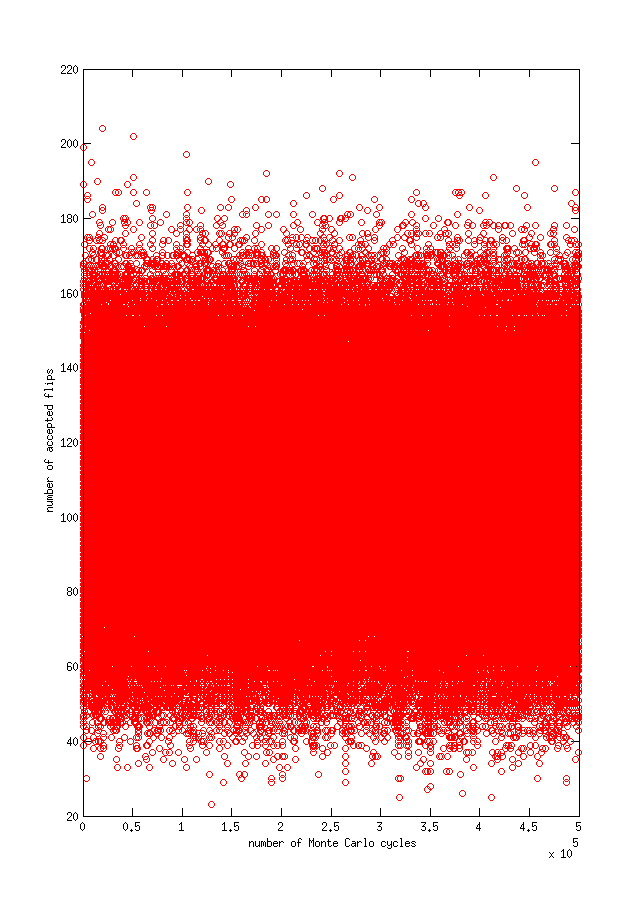
\includegraphics[scale = 0.45]{accepted_flips_temp2dot4.png}
%  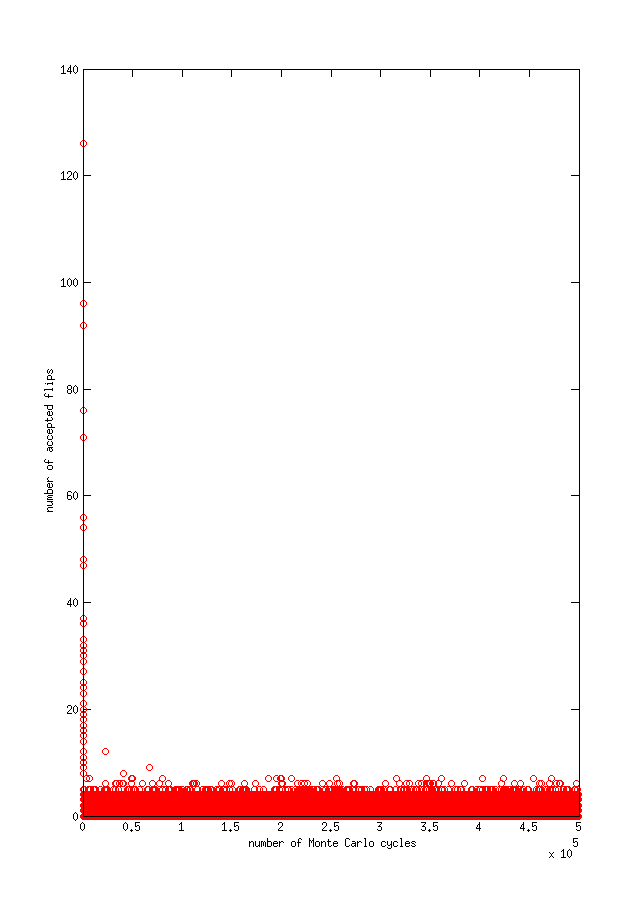
\includegraphics[scale = 0.45]{accepted_flips_temp1.png}
%  \caption{Number of accepted spin flips. T = 2.4 to the left, and T = 1 on the right.}
%  \label{both_accepted_flpis}
% \end{figure}
\section{Solving by Finite Element Methods}
The normal approach to solving partial differential equations (especially in more than one dimension) in industry is to discretize using a finite 
difference 
scheme in time, and a finite element method in space. The finite element method is quite a lot more complex both in its discretization and in its 
implementation, which is why we will use the FEniCS software pack to solve the equation using finite elements. The reason one would typically use 
finite elements for PDEs is that it easily generalizes to complex geometries with dynamic choise of resolution, and that one can choose freely how 
accurate the approximation should be.\\
Consider this a very short and superficial explaniation of the finite element method. We will stick to 1 dimension.\\
The basic idea is to map our approximation of the solution on a function space of some piecewise continous functions. That is, we divide the unit 
square, on which our equation is defined, into some number of elements. Notice that an element typically takes the form of a triangle, and that the 
elements can vary in size (for simplicity we will use elements of equal size). A triangle in one dimension is simply an interval, defined by two 
points. Theese points are called nodes. We now use the nodes to define linear functions on each element, and demand that each linear function is exactly 
1 on one node and 0 on the other. We can of course use any function we want which fulfills this cirterion, but the standard functions to use are 
some orthogonal polynomial, specifically the Lagrange polynomials (of some degree depending on the number of nodes per element). So far we have our 
equation and we have a finctionspace $V = span\{\phi_i\}$ where $\phi_i$ is the Lagrange polynomial at element number i. We discretize the equation 
in time ($u_{xx}$ denotes the duble derivative of u wrt x).
\begin{align*}
 u^{n+1}-u^n -\Delta tu^n_{xx} = 0 \\
 R = 0
\end{align*}
we now want to approximate R on V, minimizing the error. There are a few ways to do this, and again we will use a quite general one, the Galerkin 
method. To minimize the error we take the inner product $(R,V) = 0 \forall \phi_i \in V$ which leads to the following integrals
\begin{align*}
 \int_\Omega u^{n+1}\phi_id\Omega - \int_\Omega u^{n}\phi_id\Omega -\Delta t \int_\Omega u^{n}_{xx}\phi_id\Omega = 0 \\
 \int_\Omega \sum\limits_{j=1}^N(\phi_j\phi_i)u^{n+1}d\Omega - \int_\Omega \sum\limits_{j=1}^N(\phi_j\phi_i)u^{n}d\Omega -
 \Delta t \int_\Omega \sum\limits_{j=1}^N(\phi_j''\phi_i)u^{n}d\Omega = 0 
\end{align*}
where we have used the approximation of u on V $u\simeq\sum\limits_{j=1}^N\phi_ju$. We notice that taking a double derivative of $\phi_j$ leaves us 
with 0, so we try integrating it by parts
\begin{align*}
 - \Delta t \int_\Omega \sum\limits_{j=1}^N(\phi_j''\phi_i)u^{n}d\Omega = \Delta t\big([\phi_j'\phi_iu]_{\d\Omega} -\int_\Omega \sum 
 \phi_j'\phi_i'u^nd\Omega\big)
\end{align*}
which is a boundary term and a new integral. This is actually sufficient for FEniCS to work with. The rest of the computation is simply assembly of a 
linear system from the integrals, and solving the linear system.

\section{Final comments}
Even though the analysis in section \ref{stability} suggests that the Crank Nicolson scheme is supposed to have a better error than the other two, 
the results from our verification tells us that the Backward Euler scheme is better. It is also easier to implement, and it demands less FLOPS than 
the CN scheme because there is no need to make a new vector at each timestep. The Crank Nicolson scheme is also known to have some porblems with 
oscillating solutions, even though we do not see any of theese here. This is probably due to the restrictions put on $\Delta t$ from the Forward 
Euler scheme which we have used for all schemes.\\
We notice from figures (\ref{errors_nx10}) and (\ref{errors_nx100}) that the error is not quite of the order we had expected. The expected value is 
that the error goes like $\mathcal{O}(\Delta t)$ and we have $\Delta t \propto \Delta x^2$, so we should have an error of $10^{-2}$ for 
$\Delta x = 0.1$ and $10^{-4}$ for $\Delta x = 0.01$. We almost have this error, but not quite. This is telling me that there either is something 
wrong somewhere in my program, or there is an error done at some point while making the exact solution. Havinig looked over both of theese possibilities 
quite a few times, I have unfortunately yet to find this error. My perliminary explanation is that the error still is proportional to 
$\Delta t$, the proportionality-constant just happens to be 10.\\
The section on finite element methods is ment only as a short glance onward from this project into more complex problems which are still on the same 
form as this one. \\
Source code can be found in the appendix.
\end{document}
